%% ============================================================
%%  Chapter 4, Cs$_{0.1}$FA$_{0.9}$PbI$_3$ Perovskite Solar
%%              Cells as Ionizing Radiation Monitors
%%  Dissertation: Radiation Responsive Materials for Advanced
%%  Radiation Detection and Systems
%% ============================================================

\chapter{Cs$_{0.1}$FA$_{0.9}$PbI$_3$ Perovskite Solar Cells as Ionizing Radiation Monitors}
\label{ch:CsFAPbI}

The preceding chapter established that halide perovskites combine the
electronic properties requisite for radiation detection, high effective
atomic number, adequate charge-carrier mobility-lifetime products, and
tunable bandgap, with solution-processable fabrication routes
inaccessible to conventional compound semiconductors.  The work
described in this chapter exploits a distinct but complementary
strategy: rather than deploying a thick single crystal as a direct
charge-collection detector, it repurposes a photovoltaic-architecture
thin-film device as a \emph{current-mode radiation monitor}.  The
rationale is twofold.  First, modern perovskite solar cells have
reached certified power-conversion efficiencies exceeding
27\%~\cite{Li2026record}, implying that the absorber layers have been
optimized over a decade of intense materials research for the very
properties, long carrier diffusion lengths, low trap-state densities,
and efficient carrier extraction, that also govern sensitivity to
ionizing radiation.  Second, photovoltaic modules are inherently scalable
in area, enabling the construction of sensor arrays whose geometric
aperture is far larger than what is practical with single-crystal bulk
detectors, and whose short-circuit current provides a direct analog
output suitable for interfacing with standard nuclear instrumentation.

The Cs$_{0.1}$FA$_{0.9}$PbI$_3$ composition is specifically chosen
because partial substitution of cesium for formamidinium suppresses
the spontaneous $\alpha \to \delta$ phase transition of pure FAPbI$_3$
while preserving its 1.48~eV bandgap and superior charge transport
relative to MAPbI$_3$~\cite{Yi2016}.  The \emph{pin} diode device
structure (Section~\ref{sec:device_fab}) further suppresses dark
current relative to a simple ohmic-contact geometry, and its inverted
polarity places the transparent electrode on the illuminated face,
an arrangement that simultaneously enables photovoltaic operation under
sunlight and direct exposure of the perovskite absorber to externally
incident radiation.

This chapter reports visible-light temporal response measurements
(Section~\ref{sec:temporal_response}), X-ray response under pulsed
and continuous illumination (Section~\ref{sec:xray_response}),
gamma-ray response during continuous $^{137}$Cs and $^{60}$Co
irradiation including a six-day and sixteen-day stability study
(Section~\ref{sec:gamma_response}), and steady-state neutron
response measurements performed at the Ohio State University Nuclear
Reactor Laboratory (Section~\ref{sec:neutron_response}).

%% ------------------------------------------------------------
\section{Device Fabrication and Photovoltaic Performance}
\label{sec:device_fab}
%% ------------------------------------------------------------

Devices were fabricated by Prof.\ Jinsong Huang's group at the
University of North Carolina at Chapel Hill using a standard inverted
(\emph{pin}) architecture developed for high-efficiency perovskite
photovoltaics.  The composition of the absorber layer is
Cs$_{0.1}$FA(CH$_3$NH$_2$)$_{0.9}$PbI$_3$, where the 10~mol\%
Cs$^+$ substitution entropy-stabilizes the cubic $\alpha$-phase at
ambient conditions as described in Section~\ref{sec:perovskite_structure}.
Device fabrication proceeded by sequential solution deposition of the
hole transport layer, the perovskite precursor solution, the electron
transport layer, and the top metal contact onto glass/ITO substrates.
The layer stack, illustrated in Figure~\ref{fig:device_structure}, is
ITO / hole transport layer / Cs$_{0.1}$FA$_{0.9}$PbI$_3$ / electron
transport layer / Ag.

\begin{figure}[htbp]
  \centering
  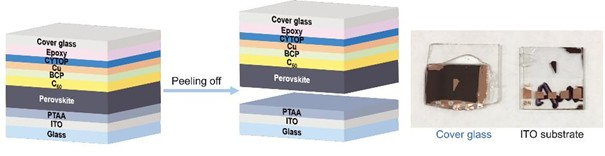
\includegraphics[width=0.60\textwidth]{figures/4_1_device_structure}
  \caption{Cross-sectional schematic of the \emph{pin} perovskite
           device structure used throughout this chapter.  The
           ITO/hole-transport-layer (HTL) contact serves as the
           illuminated face for both photovoltaic and radiation-monitoring
           operation; the Ag back contact completes the
           Cs$_{0.1}$FA$_{0.9}$PbI$_3$ absorber sandwich.}
  \label{fig:device_structure}
\end{figure}

Two device geometries were characterized: a small-area cell ($\sim$8~mm$^2$
active area) for high-throughput screening and an encapsulated module
(63.7~cm$^2$ aperture area, four cells wired in series) intended for
radiation monitoring applications.  Representative current
density--voltage (J-V) curves measured under 1-sun AM1.5G
illumination are shown in Figure~\ref{fig:pv_performance}.

\begin{figure}[htbp]
  \centering
  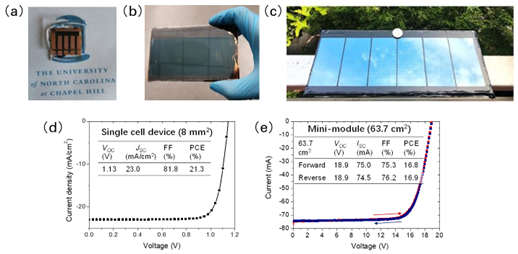
\includegraphics[width=0.85\textwidth]{figures/4_2_pv_performance}
  \caption{Photovoltaic performance of the Cs$_{0.1}$FA$_{0.9}$PbI$_3$
           devices used in this study.  (a)~J-V curve for the 8~mm$^2$
           small cell (PCE = 21.3\%, $V_{\mathrm{OC}}$ = 1.13~V,
           $J_{\mathrm{SC}}$ = 23.0~mA\,cm$^{-2}$, FF = 81.8\%).
           (b)~J-V curve for the 63.7~cm$^2$ module (PCE = 16.9\%,
           $V_{\mathrm{OC}}$ = 18.9~V, $J_{\mathrm{SC}}$ = 74.5~mA\,cm$^{-2}$,
           FF = 76.2\%).  All measurements performed at UNC Chapel Hill
           under AM1.5G illumination prior to shipment.}
  \label{fig:pv_performance}
\end{figure}

The small-cell PCE of 21.3\% is consistent with champion efficiencies
reported for the Cs$_{0.1}$FA$_{0.9}$PbI$_3$ composition in the
contemporary literature~\cite{Liu2024inverted}, confirming that the
devices received for radiation testing represent the current state of
the art in perovskite photovoltaic fabrication.  The module efficiency
of 16.9\% reflects the geometric fill-factor penalty inherent in a
series-connected configuration and is comparable to certified module
efficiencies from the same composition reported by independent
groups~\cite{Li2026record}.

%% ------------------------------------------------------------
\section{Temporal Photoresponse Characterization}
\label{sec:temporal_response}
%% ------------------------------------------------------------

Before proceeding to ionizing radiation measurements, the time-domain
photoresponse of the devices was characterized under visible light to
establish the inherent bandwidth of the detector and to identify
any device-physics limitations on pulse-following ability.  Three
complementary measurement modalities were employed: a DC chopped-beam
experiment to measure the turn-on and turn-off time constants, a
pulsed-laser experiment to probe the high-frequency limit, and an
AC-coupled grid-simulation experiment to assess the feasibility of
power-grid synchronization using the solar module.

\subsection{DC Transient Response}

The DC transient measurement used a 532~nm continuous-wave laser
attenuated to approximately 0.45 sun equivalent irradiance and modulated
by a mechanical optical chopper.  Short-circuit current transients were
acquired on a digital oscilloscope and analyzed to extract the 10--90\%
rise time and the 90--10\% fall time.

The 8~mm$^2$ cell exhibited a rise time of approximately 33~ms, while
the 28.6~cm$^2$ module required approximately 60~ms to reach 80\% of its
peak short-circuit current after the chopper opened.  Both values are
substantially longer than the RC time constants computed from the
device capacitance and load resistance, confirming that the observed
response time is limited by the chopper blade transit speed rather
than by any intrinsic device physics.  This conclusion is consistent
with the known sub-microsecond free-carrier lifetimes in high-quality
Cs--FA perovskite films~\cite{Guerrero2021chemrev}.

\subsection{Pulsed Laser Response}
\label{sec:pulsed_laser}

To access the true high-frequency bandwidth of the devices, a pulsed
diode laser (Thorlabs NPL41B, 405~nm central wavelength) was used in
place of the chopped CW source.  The laser was operated at a
repetition rate of 1~kHz with a pulse width of 20~ns (variable
6--38~ns range, up to 10~MHz maximum repetition rate).
Photoresponse pulses were amplified by a transimpedance amplifier
with $10^5$~V\,A$^{-1}$ gain and 1~MHz bandwidth before acquisition
on a Keysight MSO-X-3104T oscilloscope.

Two series-parallel module assemblies, denoted Cell~A and Cell~B,
each consisting of four Cs$_{0.1}$FA$_{0.9}$PbI$_3$ cells mounted on
a printed breadboard, were characterized.  Cell~A exhibited an output
pulse rise time of approximately 84~ns under these conditions; Cell~B
produced a comparable waveform.  The measured rise time is dominated
by the 1~MHz bandwidth of the transimpedance amplifier rather than
the device itself: the $-3$~dB amplifier bandwidth corresponds to a
rise-time limit of $0.35 / 10^6$~Hz $\approx 350$~ns, and the
shorter observed value reflects the partial bandwidth contribution of
the oscilloscope front-end and cable parasitics.  The intrinsic
device response is therefore faster than the approximately 84~ns
system-limited value, consistent with the sub-microsecond carrier
lifetimes expected from the $\mu\tau$ products typical of
Cs$_{0.1}$FA$_{0.9}$PbI$_3$ thin films reported in
Section~\ref{sec:hecht}.

\subsection{AC Grid Simulation}

To evaluate whether the solar module could track the periodic voltage
waveform produced by a single-phase power inverter, a potential
application for verifying grid integrity or synchronizing a radiation
monitor to a power-cycle reference, the four-cell module was
connected to the input of a commercial single-phase DC-to-AC
microinverter under indoor fluorescent illumination.  The inverter
consumed approximately 4~W at its rated load, but the module could
deliver only $\sim$1~W under the available illumination, leaving the
inverter operating in a deeply underloaded regime.  No distinct
50/60~Hz modulation of the module output current was discernible
above the noise floor in this configuration.  The negative result
is attributed entirely to the power deficit rather than to any
bandwidth limitation of the perovskite device: achieving an
observable AC response would require either a larger-aperture module,
a light concentrator, or a calibrated illumination source at close
to 1-sun intensity.

%% ------------------------------------------------------------
\section{X-Ray Response}
\label{sec:xray_response}
%% ------------------------------------------------------------

X-ray characterization was performed using an Amptek Mini-X miniature
X-ray tube with a gold anode, operated at tube voltages up to 50~kV.
For continuous-wave measurements, the module was placed in the
beam path and J-V characteristics were recorded as a function of
X-ray tube voltage and current.  Figure~\ref{fig:xray_iv} shows
the resulting I-V curves; the short-circuit current $I_{\mathrm{SC}}$
increases monotonically with tube voltage, consistent with the
increasing photon fluence and mean photon energy.

\begin{figure}[htbp]
  \centering
  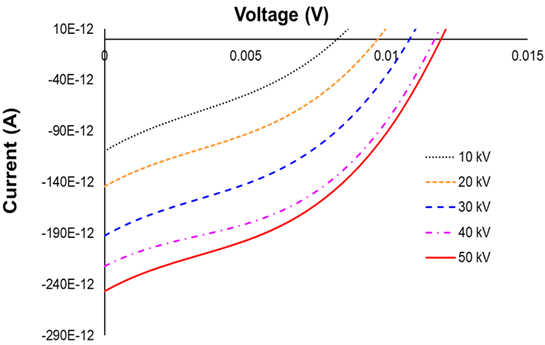
\includegraphics[width=0.70\textwidth]{figures/4_3_xray_iv}
  \caption{Current-voltage characteristics of the
           Cs$_{0.1}$FA$_{0.9}$PbI$_3$ module under Amptek Mini-X
           X-ray tube illumination at tube voltages from 10~kV to 50~kV.
           Inset: $I_{\mathrm{SC}}$ at 50~kV as a function of irradiation
           time.}
  \label{fig:xray_iv}
\end{figure}

The time-resolved $I_{\mathrm{SC}}$ at 50~kV, shown in the inset of
Figure~\ref{fig:xray_iv}, exhibits the characteristic slow-decline
behavior previously reported for perovskite photovoltaic devices
under sustained illumination in the presence of a built-in electric
field.  The decline is attributed to ion migration: mobile halide
vacancies drift under the device's built-in field, accumulating at
the charge-transport layer interfaces and partially screening the
collection field~\cite{Thiesbrummel2024ionmig,Eames2015}.

The absolute $I_{\mathrm{SC}}$ induced by the X-ray source is substantially
smaller than that observed in the silicon reference device operated under
the same conditions, owing to the much smaller active area of the
perovskite module relative to the silicon photodiode used for comparison
($\sim$64~cm$^2$ vs.\ several hundred cm$^2$).  On a per-unit-area basis,
the perovskite compares favorably due to its higher photoelectric
absorption cross section at the relevant photon energies.

For pulsed X-ray measurements, the Amptek Mini-X beam was modulated by
a Thorlabs MC2000 optical chopper equipped with a 10-slot blade
(760~$\mu$m stainless steel, slot width matched to achieve pulse
frequencies from 10~Hz to 1~kHz).  The pulsed response confirmed that
the device faithfully follows the beam modulation at frequencies up
to the chopper bandwidth, consistent with the pulsed laser measurements
in Section~\ref{sec:pulsed_laser}.

%% ------------------------------------------------------------
\section{Gamma-Ray Response}
\label{sec:gamma_response}
%% ------------------------------------------------------------

\subsection{Measurement Setup and Dose Rate Calibration}

Gamma-ray irradiation experiments were performed at the Ohio State
University Nuclear Reactor Laboratory (OSU NRL) using two
independent sources: a benchtop $^{137}$Cs irradiator
(six source rods, $E_\gamma = 662$~keV) and a $^{60}$Co irradiator
submerged in the reactor pool ($E_\gamma = 1.17$ and 1.33~MeV).
Because the dose rate calibration values provided with each irradiator
are given in units of roentgen per hour for air, conversion to the
absorbed dose rate in the perovskite film was performed using the
relation

\begin{equation}
  \dot{D}_{\mathrm{perovskite}}
    = 0.877 \times \frac{(\mu_{\mathrm{en}}/\rho)_{\mathrm{perovskite}}}
                        {(\mu_{\mathrm{en}}/\rho)_{\mathrm{Si}}}
      \times \dot{X},
  \label{eq:doserate}
\end{equation}

\noindent where $\dot{X}$ is the exposure rate in roentgen per hour,
0.877~rad/R is the roentgen-to-rad conversion factor for
soft tissue~\cite{knoll2010}, and the ratio of mass energy-absorption
coefficients $(\mu_{\mathrm{en}}/\rho)$ was evaluated at the
mean photon energy of each source using NIST XCOM tabulations~\cite{Berger2010xcom}.
This procedure yielded dose rates of 44.16~rad\,hr$^{-1}$ in the
perovskite layer for the $^{137}$Cs irradiator and 355.61~rad\,hr$^{-1}$
for the $^{60}$Co source.

\subsection{Cesium-137 Irradiation}
\label{sec:cs137}

The Cs$_{0.1}$FA$_{0.9}$PbI$_3$ module was inserted into and withdrawn
from the $^{137}$Cs irradiator while the short-circuit current was
monitored in real time.  Figure~\ref{fig:cs137_isc} shows a time-series
of $I_{\mathrm{SC}}$ recorded during a representative insert/withdraw cycle.
A clear and reproducible step change in $I_{\mathrm{SC}}$ is observed upon
insertion, with the current increasing by an amount proportional to the
gamma-induced electron-hole pair generation rate within the absorber.
The induced current density at 44.16~rad\,hr$^{-1}$ was measured as
2.19~nA\,cm$^{-2}$, which represents the net gamma-to-current conversion
sensitivity of the device under the prevailing irradiation geometry.

\begin{figure}[htbp]
  \centering
  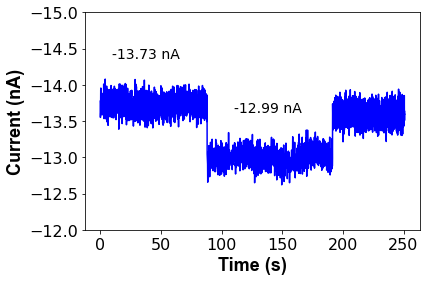
\includegraphics[width=0.80\textwidth]{figures/4_4_cs137_response}
  \caption{Short-circuit current $I_{\mathrm{SC}}$ of the
           Cs$_{0.1}$FA$_{0.9}$PbI$_3$ module as a function of time
           during insertion into and withdrawal from the $^{137}$Cs
           irradiator (dose rate = 44.16~rad\,hr$^{-1}$ in perovskite).}
  \label{fig:cs137_isc}
\end{figure}

To assess the long-term stability of the perovskite module as a
radiation monitor, the device was subjected to continuous $^{137}$Cs
irradiation for six days without removal from the source.  The
accumulated absorbed dose over the six-day period was computed by
integrating the dose rate over the irradiation time.
Figure~\ref{fig:cs137_longterm} shows the evolution of $I_{\mathrm{SC}}$
as a function of cumulative absorbed dose.  A linear decrease in
$I_{\mathrm{SC}}$ with dose is observed, with a slope of
$-0.74$~nA\,rad$^{-1}$, corresponding to a relative degradation rate
of approximately $\left[I_{\mathrm{SC}}(0) - I_{\mathrm{SC}}(D)\right] / I_{\mathrm{SC}}(0)$
per unit absorbed dose.

\begin{figure}[htbp]
  \centering
  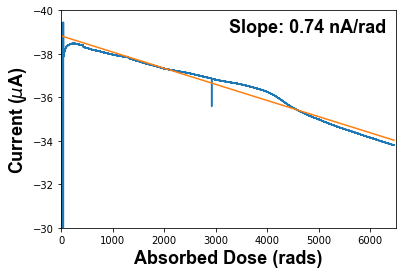
\includegraphics[width=0.80\textwidth]{figures/4_5_cs137_longterm}
  \caption{Long-term evolution of $I_{\mathrm{SC}}$ under continuous
           $^{137}$Cs irradiation (44.16~rad\,hr$^{-1}$) over six
           days.}
  \label{fig:cs137_longterm}
\end{figure}

The observed linear decline is consistent with the creation of
electrically active defects, primarily iodide Frenkel pairs,
proportional to the absorbed dose, as has been documented for
$^{60}$Co irradiation of MAPbI$_3$ single crystals at doses up to
1000~krad~\cite{Boldyreva2020gammarad}.  An additional contribution
to the $I_{\mathrm{SC}}$ decline comes from cumulative darkening of the
borosilicate glass superstrate, which reduces the visible-light
transmittance and hence the photovoltaic current even in the absence
of absorber degradation; this contribution has been documented
separately~\cite{Boldyreva2024cs137}.

\subsection{Cobalt-60 Irradiation}
\label{sec:co60}

The module was subsequently irradiated in the OSU NRL reactor pool
using the underwater $^{60}$Co irradiator at a dose rate of
355.61~rad\,hr$^{-1}$ in the perovskite layer, approximately eight
times higher than the $^{137}$Cs rate.  The measurement
geometry was otherwise identical: $I_{\mathrm{SC}}$ was recorded
continuously throughout a 16-day irradiation.  The induced current
density at 355.61~rad\,hr$^{-1}$ was 3.56~nA\,cm$^{-2}$.

Figure~\ref{fig:co60_response} shows the $I_{\mathrm{SC}}$ time series for
the $^{60}$Co irradiation.  As with $^{137}$Cs, a downward linear
trend in the baseline $I_{\mathrm{SC}}$ is observed over the 16-day
period, consistent with progressive defect accumulation proportional
to absorbed dose.

\begin{figure}[htbp]
  \centering
  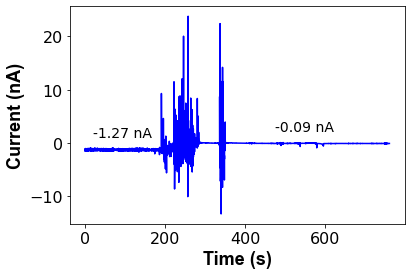
\includegraphics[width=0.80\textwidth]{figures/4_6_co60_response}
  \caption{Short-circuit current $I_{\mathrm{SC}}$ of the module during
           16-day continuous $^{60}$Co irradiation (dose rate =
           355.61~rad\,hr$^{-1}$ in perovskite).}
  \label{fig:co60_response}
\end{figure}

These results demonstrate that arrays of calibrated perovskite modules
could, in principle, be deployed in a spatial configuration around a
radiation source to triangulate the detonation location or measure
the spatial dose distribution by comparing the $I_{\mathrm{SC}}$ responses
of individual array elements.  The linear dose--current relationship
established here provides the calibration function necessary for
such an application.

%% ------------------------------------------------------------
\section{Neutron Response}
\label{sec:neutron_response}
%% ------------------------------------------------------------

Neutron response measurements were performed at the Fast Neutron
Beam Facility (FBF) of the Ohio State University Research Reactor
(OSURR).  The FBF beamline and its filtering elements are
described in full in Section~\ref{sec:osurr_fbf} below; the
experimental geometry for the solar-cell measurements placed the
perovskite module alternately outside the beam (background), in
the beam with the gamma-suppression filter closed, and in the beam
with the filter open, enabling separation of the neutron-induced
and gamma-induced current components.

%% ------------------------------------------------------------
\subsection{OSURR Fast Neutron Beam Facility}
\label{sec:osurr_fbf}
%% ------------------------------------------------------------

The OSURR is a 500-kW$_{\mathrm{th}}$ pool-type research reactor
operated by the OSU Nuclear Reactor Laboratory.  The Fast Neutron
Beam Facility (FBF) is a horizontal beamport extending from the
reactor core through the biological shielding to an experimental
area, providing access to the reactor's fast and epi-thermal
neutron flux for detector characterisation.  The beam line
contains three independently configurable filtering elements,
each of which modifies the fast neutron flux and gamma dose rate
reaching the detector in a distinct way.

The first element is a permanent 4-inch (10.16~cm) single-crystal
bismuth block embedded near the reactor core as an in-line gamma
filter.  Bismuth is nearly transparent to fast neutrons while
strongly attenuating the intense prompt fission gamma flux
produced by the reactor core.  This filter is always in place
and is not removable during experiments.

The second element is an 8-inch (20.32~cm) lead gamma shutter
embedded in the reactor's concrete shielding wall downstream of
the bismuth filter.  The shutter consists of a cylindrical drum
filled with $\tfrac{1}{16}$-inch (0.159~cm) Pb shot.  When open,
the neutron beam passes through an air gap in the drum; when
closed, the beam traverses the full column of lead shot,
providing approximately 8~inches of gamma shielding in total.
Closing the gamma shutter reduces the gamma-ray content of the
beam by a factor of 300, while simultaneously attenuating the
fast neutron flux by a factor of 35.  With the shutter open and
no cadmium filter in place, the fast neutron flux at the detector
position is $1.5\times10^7$~cm$^{-2}$\,s$^{-1}$ and the gamma
dose rate is 15.787~R\,hr$^{-1}$.  With the shutter closed, the
fast neutron flux drops to $4.3\times10^5$~cm$^{-2}$\,s$^{-1}$
and the gamma dose rate falls to 50.525~mR\,hr$^{-1}$.

The third element is an external 2-mm cadmium (Cd) foil
positioned at the beam exit port.  Cadmium has a very large
absorption cross-section for thermal neutrons (below
$\sim$0.5~eV) and acts as a selective thermal neutron filter,
leaving the fast and epi-thermal components of the beam largely
unaffected.  The Cd foil was characterised via gold foil
activation measurements per ASTM E262-17, yielding a Cadmium
Ratio of 1.1 and a thermal neutron reduction factor of 110.
When the gamma shutter is closed and the Cd filter is inserted,
the estimated thermal neutron flux at the detector is reduced to
$\sim$220~cm$^{-2}$\,s$^{-1}$, while the fast neutron flux
remains at $4.3\times10^5$~cm$^{-2}$\,s$^{-1}$.  The combined
effect of all three filtering configurations on the beam
composition is summarised in Table~\ref{tab:fbf_beam_ch4}.

\begin{table}[htbp]
\centering
\caption{OSURR FBF beam conditions as a function of gamma shutter
         and Cd filter configuration.  All flux and dose-rate
         values are referenced to 450~kW$_{\mathrm{th}}$ reactor power
         at the detector position.}
\label{tab:fbf_beam_ch4}
\startsinglespace
\begin{tabular}{llcc}
\hline
Shutter & Cd filter & Fast neutron flux (cm$^{-2}$\,s$^{-1}$)
        & Gamma dose rate \\
\hline
Open   & Out & $1.5\times10^7$ & 15.787~R\,hr$^{-1}$  \\
Closed & Out & $4.3\times10^5$ & 50.525~mR\,hr$^{-1}$ \\
Closed & In  & $4.3\times10^5$ & 50.525~mR\,hr$^{-1}$ \\
\hline
\end{tabular}
\end{table}

The neutron energy spectrum at the FBF, determined by the SAND-II
and STAYSL spectrum-unfolding techniques using activation of
copper, gold, and nickel wire dosimeters, is shown in
Figure~\ref{fig:fbf_spectrum_ch4}.  The spectrum spans thermal
energies through the fast fission continuum, with the fast and
epi-thermal components dominating the integrated flux.  The
addition of the Cd filter has a minor effect on the spectral
shape above $\sim$1~eV and does not appreciably alter the
fast-neutron component.

\begin{figure}[htbp]
  \centering
  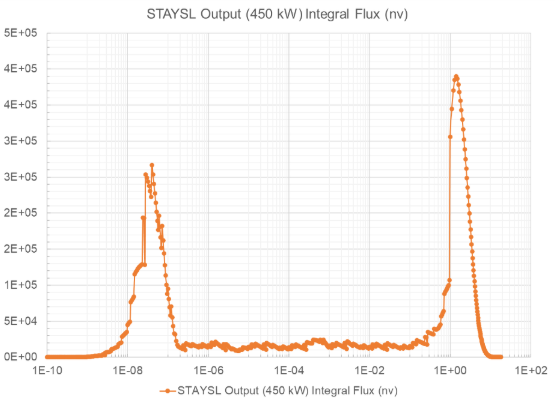
\includegraphics[width=0.75\textwidth]{figures/5_mhy_neutron_spectrum}
  \caption{Neutron energy spectrum at the OSURR FBF determined by
           SAND-II and STAYSL unfolding of Cu, Au, and Ni activation
           wire measurements.  The same spectrum applies to both the
           Cs$_{0.1}$FA$_{0.9}$PbI$_3$ solar-cell neutron experiments
           described in this chapter and the MHyPbCl$_3$ fast-neutron
           detection experiments described in
           Chapter~\ref{ch:MHyPbCl3}.}
  \label{fig:fbf_spectrum_ch4}
\end{figure}

\subsection{Steady-State Reactor Measurements}
\label{sec:neutron_dc}

Table~\ref{tab:neutron_steady} summarizes the short-circuit current
$I_{\mathrm{SC}}$ measured under each condition, referenced to reactor
power levels of 0~kW$_{\mathrm{th}}$ (reactor shutdown) and
450~kW$_{\mathrm{th}}$ (operating power).

\begin{table}[htbp]
\centering
\caption{Steady-state short-circuit current of the
         Cs$_{0.1}$FA$_{0.9}$PbI$_3$ module at OSU NRL FBF.
         Uncertainties are $\pm 1\sigma$ over the measurement interval.
         ``Gamma filter closed'' and ``gamma filter open'' refer to the
         polyethylene/lead shielding assembly that preferentially
         attenuates the reactor gamma flux while transmitting fast
         neutrons.}
\label{tab:neutron_steady}
\startsinglespace
\begin{tabular}{lcc}
\hline
Condition & Reactor Power & $I_{\mathrm{SC}}$ (pA) \\
\hline
Background (reactor off)  & 0 kW$_{\mathrm{th}}$   & $51.29 \pm 6.60$  \\
Background (reactor on)   & 450 kW$_{\mathrm{th}}$ & $57.50 \pm 7.39$  \\
Gamma filter closed       & 450 kW$_{\mathrm{th}}$ & $57.62 \pm 7.93$  \\
Gamma filter open         & 450 kW$_{\mathrm{th}}$ & $59.77 \pm 8.62$  \\
\hline
\end{tabular}
\end{table}

The data in Table~\ref{tab:neutron_steady} reveal a slight but
statistically marginal increase in $I_{\mathrm{SC}}$ upon opening the gamma
filter (from $57.62 \pm 7.93$~pA to $59.77 \pm 8.62$~pA).  The
difference of $\sim$2.2~pA represents a $\sim$0.26$\sigma$ effect
relative to the combined quadrature uncertainty, which is not
statistically significant at the 95\% confidence level.  The result is
therefore classified as inconclusive: a neutron-induced contribution
cannot be ruled out, but the signal-to-noise ratio of a single
8~mm$^2$--63.7~cm$^2$ module is insufficient to resolve it above the
fluctuating gamma and ambient backgrounds present at the FBF port.

These results motivate the use of a larger-area array for future
neutron sensing experiments.  Scaling the active area by a factor of
ten to twenty, combined with the differential signal extraction method
described by Panaccione et al.~\cite{Panaccione_NIM_2024}, is expected
to raise the neutron-to-background ratio above the detection threshold.

\subsection{Chopped-Beam Transient Measurements}

In an attempt to resolve a time-modulated neutron signal against the
steady-state gamma background, the reactor beam was mechanically
chopped at frequencies between 1~Hz and 100~Hz using a borated
polyethylene blade.  Synchronous detection (lock-in analysis) of the
$I_{\mathrm{SC}}$ transient was implemented in software.  No neutron-induced
current component was detected above the noise floor under any chopping
frequency in this configuration, consistent with the steady-state
analysis: the signal magnitude is simply too small relative to the
electronic noise of the current measurement system at the flux levels
available from the 450~kW$_{\mathrm{th}}$ reactor at the FBF port.
\section{Summary}
\label{sec:ch4_summary}
%% ------------------------------------------------------------

This chapter has demonstrated that photovoltaic-architecture
Cs$_{0.1}$FA$_{0.9}$PbI$_3$ perovskite solar cells can serve as
sensitive current-mode monitors for a broad spectrum of ionizing
radiation.  The key results are as follows.

Temporally, the device bandwidth is limited by the measurement
electronics rather than the intrinsic perovskite photoresponse:
rise times of 33--84~ns were recorded depending on the amplifier
configuration, and the actual carrier lifetime in the film is
substantially shorter than the measured system rise time.

Under X-ray irradiation (Amptek Mini-X, up to 50~kV), the module
produces a measurable short-circuit current proportional to the
beam intensity, with the characteristic slow $I_{\mathrm{SC}}$ decline
associated with ion-migration field screening under the device's
built-in field~\cite{Thiesbrummel2024ionmig}.

Under $^{137}$Cs gamma irradiation at 44.16~rad\,hr$^{-1}$,
an induced current density of 2.19~nA\,cm$^{-2}$ was measured,
and a distinct step response was observed upon insertion and
withdrawal.  Long-term (six-day) continuous irradiation revealed a
linear decline of $\sim$0.74~nA\,rad$^{-1}$ attributable to
cumulative defect creation and glass darkening~\cite{Boldyreva2020gammarad,Boldyreva2024cs137}.
The $^{60}$Co measurement at 355.61~rad\,hr$^{-1}$ yielded
3.56~nA\,cm$^{-2}$ and an equivalent linear degradation trend over
sixteen days, confirming the scalability of the current-mode detection
approach across a dose-rate range spanning nearly an order of magnitude.

Neutron response at the OSU NRL FBF was statistically inconclusive
for a single module at 450~kW$_{\mathrm{th}}$; the signal-to-noise
analysis indicates that scaling the detector array area by a factor
of ten to twenty is necessary to resolve the neutron-induced current
above the combined gamma and electronic noise backgrounds.